\chapter{Parameter Reconstruction}
\label{ch:ParamRecon}


%A common problem in physics is attempting to reconstruct the parameters of a model from a set of data. Stated more precisely, this is an attempt to answer the following question: given a set of data $\mathcal{D}$, what is the probability of a given set of model parameters $\boldsymbol\theta$ being the true, underlying parameters? But how do we interpret this question and what do we mean by the `probability' of a given set of parameters?

In this appendix, we address the problem of parameter reconstruction. Given a set of data $\mathcal{D}$, we would like to make some statement about the values of a set of model parameters $\boldtheta$. Due to statistical and systematic uncertainties, this will be a probabilistic statement about which values of $\boldtheta$ are more likely. Here, we consider what is meant by `more likely'. We then demonstrate how parameter estimates and uncertainty intervals are constructed and how the parameter space of $\boldtheta$ can be explored to obtain these estimates.

In general, there are two approaches to parameter estimation. In \textit{frequentist} inference, there is only a single, fixed set of true values for the model parameters $\boldsymbol\theta$. We imagine that the experiment (which produced the data $\mathcal{D}$) can be repeated a large number of times, giving independent results each time. The `probability' associated with each set of parameters $\boldsymbol\theta$ is a measure of how frequently our experiment would produce data which looked similar to $\mathcal{D}$ if $\boldsymbol\theta$ are the true parameter values. In a frequentist framework, the true model parameters are fixed but unknown and we make statements about how confident we are that these true parameters lie in a particular range.

An alternative approach is \textit{Bayesian} inference. The true parameter value is treated as a random variable and we use Bayes' theorem to determine its probability distribution from the data:
\begin{equation}
P(\boldsymbol\theta|\mathcal{D}) = P(\boldsymbol\theta) \frac{P(\mathcal{D}|\boldsymbol\theta)}{P(\mathcal{D})}\,.
\end{equation}
In doing so, we need to know $P(\boldsymbol\theta)$, known as the prior on the model parameters. This is a measure of our beliefs about the true value of $\boldsymbol\theta$ and may be motivated by theoretical considerations or information from other experiments. In a Bayesian framework, we combine the data with information about our prior expectations to make statements about the probability of $\boldsymbol\theta$ having a particular value.

%These two approaches have different strengths and weaknesses, as we shall explore, and have both been applied to the problem of parameter exploration in physics. In this chapter, we will discuss how both frequentist and Bayesian statistics are used to make parameter estimates and measure the degree of certainty in these estimates. We will describe several methods which are used to explore parameter spaces and therefore make parameter inferences. Finally, we will outline how to calculate the likelihood $\mathcal{L}$ - the probability of obtaining a particular set of data given some underlying model parameters - which is at the core of both the frequentist and Bayesian approaches.

%Plan for this chapter:
%-`Shape of a parameter space' - define the likelihood and the posterior distribution (and marginalisation/profiling)
%-`Estimates' - what do we do for point estimates and spread estimates
%-`Methods' - MCMC and Nested Sampling
%-`Likelihood examples' - some likelihoods, such as poisson and extended (so that I don't have to do them later)


\section{Frequentist statistics}

%\subsection{Likelihoods}

In frequentist statistics, the most important quantity to consider is the \textit{likelihood} of a given point in parameter space, $\mathcal{L}(\boldsymbol\theta)$, defined as the probability of obtaining the data $\mathcal{D}$, assuming that $\boldsymbol\theta$ is the true parameter value. The likelihood often takes a very small value (because the probability of obtaining a particular data set out of all possible data sets is typically very small), and so it is convenient to work with the log-likelihood $l(\boldtheta) = \ln(\mathcal{L}(\boldtheta))$. The absolute value of $\mathcal{L}(\boldsymbol\theta)$ carries no significance. However, the likelihood value of a particular point, relative to another, can be interpreted as a measure of the relative goodness of fit of the points. While the likelihood is not a probability distribution, in the limit of a large number of samples $l(\boldtheta)$ follows a $\chi^2$ distribution (as we shall discuss shortly) and therefore can have a probabilistic interpretation.

Often, we may not be interested in all of the parameters of $\boldtheta$. For example, we may partition the parameters into parameters of interests $\boldpsi$ and so-called nuisance parameters $\boldphi$: $\boldtheta = (\boldpsi, \boldphi)$. These nuisance parameters may be parameters which we are not directly interested in, but which must be included in the analysis to account for all the relevant uncertainties. We often want to reduce the dimensionality of $\boldtheta$ to consider only how the likelihood varies as a function of $\boldpsi$.

One method of doing this is by maximizing the full likelihood function over the nuisance parameters:
\begin{equation}
\label{eq:parameter:profilelikelihood}
\mathcal{L}_p(\boldsymbol{\psi}) = \max_{\boldsymbol{\phi}} \mathcal{L}(\boldsymbol{\psi},\boldsymbol{\phi})\,.
\end{equation}
That is, for each value of $\boldpsi$, we select the maximum value of $\mathcal{L}$ obtained from all possible values of $\boldphi$. This projection onto the subset of parameters $\boldpsi$ is referred to as the profile likelihood.

An alternative method of reducing the dimensionality of the full parameter space is to calculate the mean likelihood:
\begin{equation}
\label{eq:parameter:meanlikelihood}
\mathcal{L}_m(\boldsymbol{\psi}) = \frac{\int \mathcal{L}(\boldpsi, \boldphi) \, \mathrm{d}\boldphi}{\int \, \mathrm{d}\boldphi}\,.
\end{equation}
The mean likelihood allows us to take into account the structure of the likelihood function in the nuisance directions. The profile likelihood simply selects the largest likelihood value at each value of $\boldpsi$, even if this value is only realised over a small range of values in $\boldphi$. By comparison, the mean likelihood receives a greater contribution from wide ranges of $\boldphi$ which have a moderate likelihood value. The profile likelihood is more typically used in the literature.

\subsection{Parameter estimates}
\label{sec:ParamRecon:freqparams}
In frequentist statistics, the point estimate of a parameter is relatively unambiguous. This point estimate is given by the best fit point, or maximum likelihood estimate (MLE), $\hat{\boldtheta}$, such that:
\begin{equation}
\max \mathcal{L}(\boldtheta) = \mathcal{L}(\hat{\boldtheta})\,.
\end{equation}
This estimate is the same whether we use the full likelihood or the profile likelihood, while using the mean likelihood may lead to a different value. In parameter inference, it is useful to consider the relative log-likelihood $l_r$:
\begin{equation}
l_r(\boldtheta) = \ln\left(\frac{\mathcal{L}(\boldtheta)}{\mathcal{L}(\hat{\boldtheta})}\right)\,.
\end{equation}
The logarithm is a monotonically increasing function and therefore the maximum of the likelihood and the relative log-likelihood are obtained for the same parameter values $\hat{\boldtheta}$. According to Wilks' theorem \cite{Wilks:1938}, $l_r$ is asympototically $\chi^2$-distributed as the number of samples $N$ in the data tends to infinity,

\begin{equation}
-2l_r \sim \chi^2_k\,,
\end{equation}
where the number of degrees of freedom $k$ is equal to the dimensionality of the space $\boldpsi = \left(\psi_1,...,\psi_k\right)$. This asymptotic behaviour applies equally well for the full likelihood and the profile likelihood \cite{Biller:2014} and allows us to construct confidence intervals.

We construct a $p\%$ interval from all values of $\boldpsi$ for which
\begin{equation}
l_r(\boldpsi) \leq -\frac{1}{2} \gamma(p\%;k)\,,
\end{equation}
where $\gamma(p\%;k)$ satisfies
\begin{equation}
\int_{0}^{\gamma(p\%;k)} P(\chi^2_k)\,\mathrm{d}\chi^2_k = p\%\,,
\end{equation}
and $P(\chi^2_k)$ is the $\chi^2_k$ probability distributon function. This is essentially a relative goodness-of-fit test. Values of $\boldpsi$ outside this interval are unlikely to produce data similar to $\mathcal{D}$ and would be rejected at the $p\%$ level in favour of the hypothesis $\boldpsi = \hat{\boldpsi}$. Equivalently, in terms of the likelihood, we include values of $\boldpsi$ for which
\begin{equation}
\mathcal{L}(\boldpsi) \geq \exp\left(-\frac{1}{2} \gamma(p\%;k)\right) \mathcal{L}(\hat{\boldpsi})\,.
\end{equation}
This is illustrated in Fig.~\ref{fig:parameter:likelihood} for the case of a single parameter of interest.

\begin{figure}[t]
\centering
  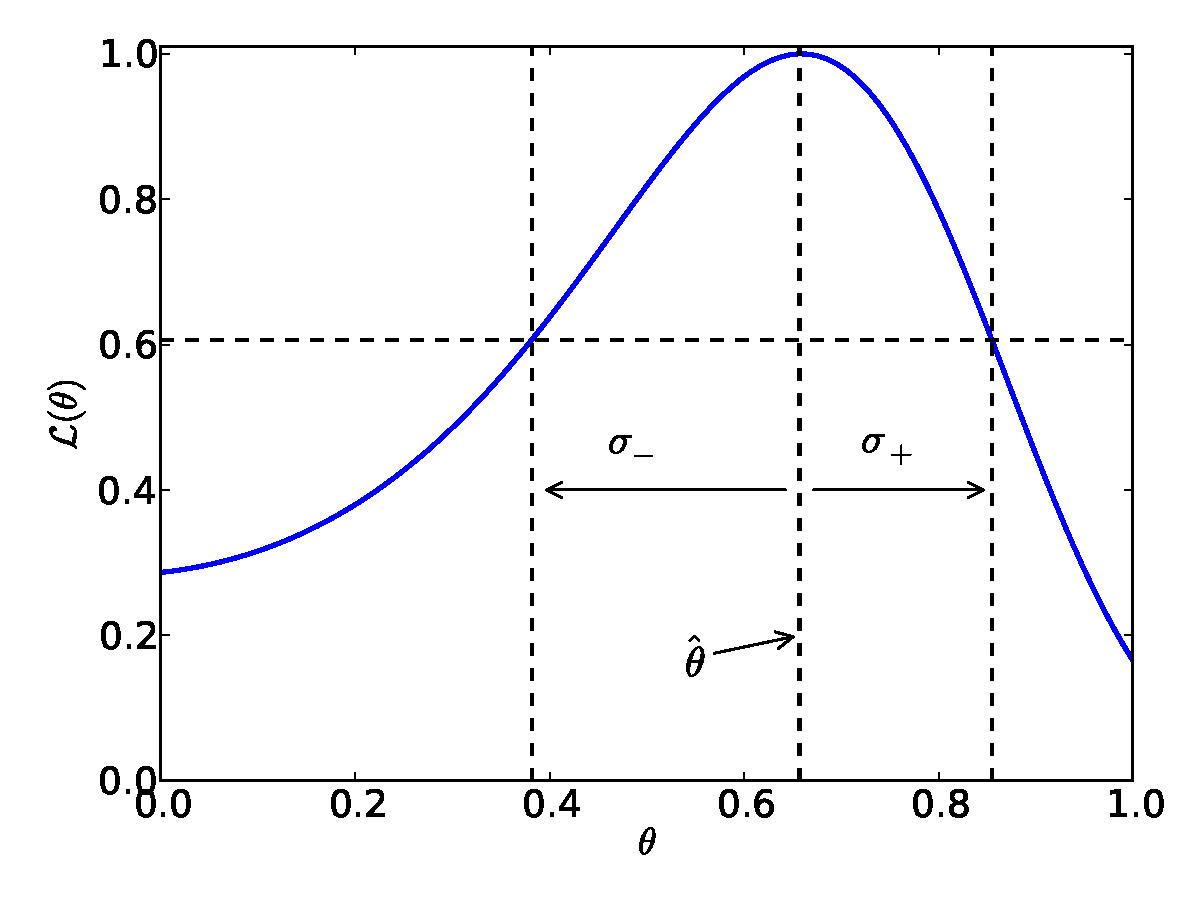
\includegraphics[width=0.8\textwidth]{ParamRecon/Likelihood.pdf}
  \caption[Likelihood-based parameter inference]{Illustration of likelihood-based parameter inference. The point estimate for the parameter $\psi$ is given by the best fit point $\hat{\psi}$. The 68\% confidence interval is given by $\psi \in [\hat{\psi} - \sigma_-, \hat{\psi} + \sigma_+]$.}
  \label{fig:parameter:likelihood}
\end{figure}



\section{Bayesian statistics}

In Bayesian statistics, we wish to obtain the \textit{posterior} probability distribution $\mathcal{P}(\boldtheta) = P(\boldsymbol\theta|\mathcal{D})$. This is obtained from Bayes' theorem:
\begin{equation}
\mathcal{P}(\boldtheta) = P(\boldsymbol\theta|\mathcal{D}) = P(\boldsymbol\theta) \frac{P(\mathcal{D}|\boldsymbol\theta)}{P(\mathcal{D})}\,.
\end{equation}
Here $P(\mathcal{D})$ is the probability of obtaining the data $\mathcal{D}$. However, this does not depend on the theoretical parameters $\boldtheta$ and we can therefore take it as an overall normalising factor for the probability distribution. The likelihood enters into the Bayesian framework as the probability of the data given the model parameters $P(\mathcal{D}|\boldsymbol\theta) = \mathcal{L}(\bold\theta)$. Finally, the prior $P(\boldsymbol\theta)$ encodes our \textit{a priori} knowledge about the true value of $\boldtheta$. If the value of a parameter, say $\theta_1$, is known to be approximately $\theta_1 = \hat{\theta}_1 \pm \sigma_\theta$, we may choose a Gaussian prior to reflect this:
\begin{equation}
P(\theta_1) \propto \exp\left(-\frac{(\theta_1 - \hat{\theta}_1)^2}{2\sigma_\theta^2}\right)\,.
\end{equation}
Alternatively, we may have a very limited knowledge of $\theta_1$ and may choose a linear-flat or log-flat prior over some range of values: $P(\theta_1) \propto 1$ or $P(\log(\theta_1)) \propto 1$. In the case of a linear-flat prior, $\mathcal{P}(\boldtheta) = \mathcal{L}(\theta)$ and the Bayesian and frequentist frameworks coincide. In contrast to the likelihood, the posterior distribution is considered a probability distribution, even in the case of small numbers of samples.

As in the frequentist case, we may wish to reduce the dimensionality of the parameter space to include only those parameters of interest $\boldpsi$. When dealing with the posterior probability, this is typically done by marginalisation. The marginalised posterior $\mathcal{P}_m$ is obtained by integrating over the nuisance parameters:

\begin{equation}
\mathcal{P}_m(\boldpsi) = \int \mathcal{P}(\boldpsi, \boldphi) \, \textrm{d}\boldphi\,.
\end{equation}
Just as $\mathcal{P}$ is a probability distribution function for the parameters $\boldtheta$, $\mathcal{P}_m$ is a probability distribution function for the parameters of interest $\boldpsi$ - specifically, the marginalised probability distribution.

\subsection{Parameter estimates}

In contrast to the frequentist case, there are several possibilities for a point parameter estimate. Because $\mathcal{P}$ and $\mathcal{P}_m$ are probability distributions, they can be described by several location parameters:

\begin{description}
\item[Mode] - the mode of the probability distribution is the value of $\boldtheta$ which maximises $\mathcal{P}$. This is also known as the maximum a posteriori (MAP) estimate and can be viewed as analogous to the maximum likelihood estimator.
\item[Median] - the median value of the parameter $\theta$ satisfies
\begin{equation}
\int_{-\infty}^{\theta_\textrm{median}} \mathcal{P}(\theta) \, \mathrm{d}\theta = \frac{1}{2}\,.
\end{equation}
This means that there is as much probability density below $\theta_\textrm{median}$ as above.
\item[Mean] - the mean value $\langle \boldtheta \rangle$ is given by
\begin{equation}
\langle \boldtheta \rangle = \int \boldtheta \mathcal{P}(\boldtheta) \, \mathrm{d}\boldtheta\,.
\end{equation}
\end{description}
Each of these will behave differently for different posterior probability distributions. The MAP estimate indicates where the greatest probability density is and may be useful when the posterior is sharpy peaked. The mean and median better reflect the global properties of the posterior probability, but may be misleading if the distribution is multimodal.


We also wish to make statements about the possible range of values for parameters. In a Bayesian framework, we define the p\% \textit{credible} interval $\mathcal{C}_{p}$ such that it encloses p\% of the probability distribution. Again, there are several possibilities for how to define $\mathcal{C}_{p} = [\mathcal{C}_{p}^\textrm{min}, \mathcal{C}_{p}^\textrm{max}]$, such as:
\begin{description}
\item[Central interval] - the interval which has the mean as its central value,
\item[Equal tails interval] - the total probability below the interval is the same as above the interval,
\begin{equation}
\int_{-\infty}^{\mathcal{C}_{p}^\textrm{min}} \mathcal{P}(\boldtheta) \, \mathrm{d}\boldtheta = \int_{\mathcal{C}_{p}^\textrm{max}}^{\infty} \mathcal{P}(\boldtheta) \, \mathrm{d}\boldtheta\,,
\end{equation}
\item[Highest density interval] - the interval defined by all values $\mathcal{P}(\theta) \geq \gamma$, where $\gamma$ is defined by
\begin{equation}
\int_{\mathcal{P}(\theta \geq \gamma)} \mathcal{P}(\boldtheta) \, \mathrm{d}\boldtheta = p\%\,.
\end{equation}
\end{description}
Highest density intervals are useful when $\mathcal{P}(\boldtheta)$ is multimodal and disjoint intervals may be required. Again, when we specify a credible interval, we must specify which definition we are using. These definitions can also be extended simply to the case where the parameter space of interest has a higher dimension. In Fig.~\ref{fig:parameter:PDF}, we illustrate the MAP estimate and mean for a hypothetical posterior distribution. We also show the 95\% credible interval obtained using the equal tails method.

\begin{figure}[t]
\centering
  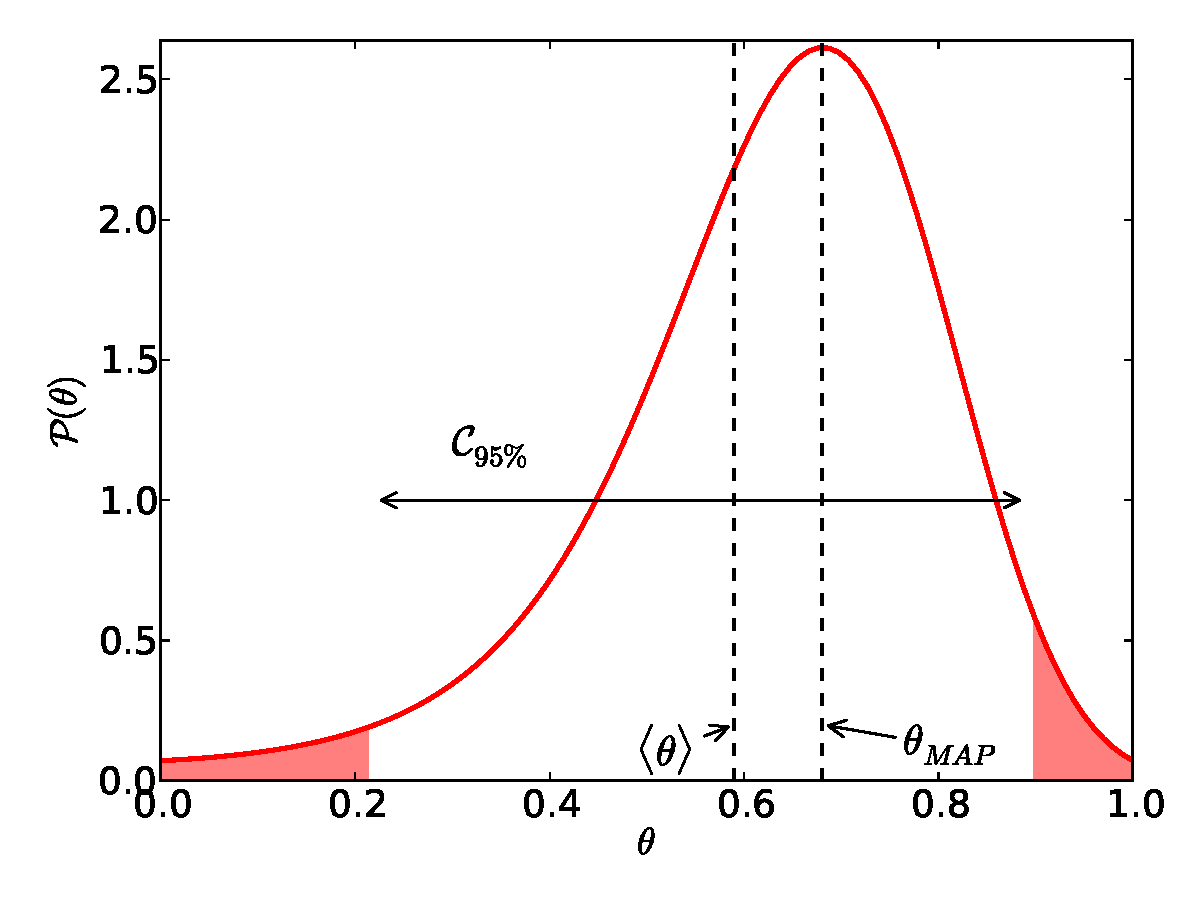
\includegraphics[width=0.8\textwidth]{ParamRecon/PDF.pdf}
  \caption[Posterior-based parameter inference]{Illustration of posterior-based parameter inference. We show the difference between the MAP and mean parameter estimates. We also show one possible 95\% credible interval - the probability in the shaded tails is equal.}
  \label{fig:parameter:PDF}
\end{figure}


\section{Exploring the parameter space}

So far we have considered how, given $\mathcal{L}(\boldtheta)$ or $\mathcal{P}(\boldtheta)$, we can make parameter inferences about $\boldtheta$. However, we have not so far considered how we can evaluate these functions. We do not typically know \textit{a priori} where $\mathcal{L}(\boldtheta)$ or $\mathcal{P}(\boldtheta)$ are maximised or what shape they have. In this section, we will briefly discuss two methodologies for mapping out these functions: Markov Chain Monte Carlo and Nested Sampling.

\subsection{Markov chain monte carlo}


In the Markov chain monte carlo (MCMC) method \cite{Lewis:2009}, we generate a chain of points in the parameter space $\left\{\boldtheta_i\right\}$. A new point $\boldtheta_{j+1}$ in the chain is generated from the current point $\boldtheta_{j}$ by picking from some proposal distribution $q(\boldtheta_{j+1}; \boldtheta_{j})$. Under the Metropolis-Hastings algorithm \cite{Metropolis:1953}, the new point is accepted with probability
\begin{equation}
\textrm{min}\left\{1, \frac{\mathcal{P}(\boldtheta_{j+1})q(\boldtheta_{j+1};\boldtheta_{j})}{\mathcal{P}(\boldtheta_{j})q(\boldtheta_{j};\boldtheta_{j+1})} \right\}\,.
\end{equation}
Over a large number of points, the chain positions should converge to a stationary distribution. Eventually the number density of chain positions will be proportional to the posterior \(n(\boldtheta) \propto \mathcal{P}(\boldtheta)\) (assuming that the proposal distribution is symmetric). In addition, we will also have the value of the likelihood $\mathcal{L}(\boldtheta)$ evaluated at all of the points in the chain.

Care must be taken to ensure that the chain has converged before the results can be interpreted. Typically some initial set of points is discarded as `burn-in', after which the chain is deemed to have converged. However, it is often unclear when convergence has been reached. Moreover, each chain position will depend slighly on the previous position. However, we want to obtain independent samples from the posterior distribution. Therefore, the chain is typically thinned (by some factor of order 25-50) \cite{Lewis:2002}, with only some of the positions being retained. Finally, we must select how many positions we want to obtain in the chain before we stop the random walk, in the hope that the chain has adequately explored the parameter space.

When $\mathcal{P}(\boldtheta)$ is multimodal, sharply peaked or has strong degeneracies among the parameters, exploration by the chain can be slow. It can be unclear whether convergence has been achieved, especially if the chain becomes trapped in one of the modes of the distribution. One way to improve the rate of convergence is to use high temperature MCMC \cite{Kirkpatrick:1983,Lewis:2009}. We employ a `heated' chain with temperature $T = 2$, meaning that we accept new points with probability
\begin{equation}
\textrm{min}\left\{1, \left(\frac{\mathcal{P}(\bold\theta_{j+1})q(\bold\theta_{j+1})}{\mathcal{P}(\bold\theta_{j})q(\bold\theta_{j})}\right)^{1/T} \right\}\,.
\end{equation}
We are now effectively sampling from a flatter posterior distribution, which allows a more rapid mixing and convergence of the chain. However, to achieve the same precision as in the $T=1$ case, we require a larger number of samples. The distribution of chain positions obtained at the higher temperature is then \(n_\textrm{T}(\boldtheta) \propto \mathcal{P}^{1/T}(\boldtheta)\). We recover the distribution of positions at \(T=1\) by `cooling' the chain:

\begin{equation}
n(\boldtheta) = n_\textrm{T}(\boldtheta) \left(\mathcal{P}(\boldtheta)\right)^{1 - 1/T}.
\end{equation}


One popular, publicly available MCMC code is \textsc{CosmoMC} \cite{Lewis:2002}. This was developed in the context of cosmological parameter estimation, but can be used as a generic MCMC sampler. When the parameter space is of a high dimension or has a number of modes, MCMC methods may prove slow. Such methods also rely on a suitable choice of burn-in and thinning factors, as well as a determination of whether convergence has occurred. Next, we explore an alternative method for efficiently obtaining samples from the posterior distribution.

\subsection{Nested sampling}

The nested sampling method \cite{Skilling:2004} was originally proposed as a method of calculating the overall normalising factor which appears in Bayes' theorem, $P(\mathcal{D})$. However, it produces as a by-product samples from the posterior distribution and values of the likelihood function. In nested sampling, we take an initial sample of points (so-called `live' points) from the parameter space and evaluate the likelihood at each point. At each subsequent step, the live point with the lowest likelihood $\mathcal{L}_0$ is removed from the sample and replaced with another point sampled from the parameter space with $\mathcal{L}_i > \mathcal{L}_0$. Thus, the algorithm explores the prior in concentric shells of $\mathcal{L}$. Each new live point can be assigned a weight $w_i$, obtained from an estimate of the change in the prior volume between concentric shells. Finally, each point can then be assigned a posterior density

\begin{equation}
p_i = \frac{w_i \mathcal{L}_i}{\mathcal{Z}}\,.
\end{equation}
The Bayesian evidence $\mathcal{Z} \equiv P(\mathcal{D})$ is obtained by summing $\sum_i w_i \mathcal{L}_i$ and the algorithm continues until this is determined to some desired precision.

In order to continue, we must be able to select points from the prior subject to the hard constraint $\mathcal{L}_i > \mathcal{L}_0$. As the algorithm moves to higher values of $\mathcal{L}_0$, points with a higher likelihood than this tend to become localised in very small regions of the parameter space. In addition, if the likelihood is multimodal or has pronounced degeneracies, the sampling of points subject to this constraint becomes highly inefficient. The \textsc{MultiNest} algorithm \cite{Feroz:2007,Feroz:2008,Feroz:2014} uses multimodal, ellipsoidal nested sampling to improve performance. As $\mathcal{L}_0$ increases during the calculation,  \textsc{MultiNest} uses the current live points to approximate the isolikelihood contour by a series of ellipsoidal surfaces. New points are drawn only from within these ellipsoids, increasing the efficiency of the sampling but still ensuring that the constraint $\mathcal{L}_i > \mathcal{L}_0$ is satisfied. The algorithm can also accommodate multiple modes in the posterior which can be explored independently.

In utilising the MultiNest algorithm, we must decide how many live point to use $N_\textrm{live}$. This determines how closely the isolikelihood contours can be followed, how dense the posterior samples will be and, in the case where there are highly localised modes, how well explored the prior will be. We must also decide the tolerance of the algorithm, \texttt{tol}. This determines the precision with which $\mathcal{Z}$ should be determined and therefore how high up the likelihood surface the algorithm should explore. Finally, we can introduce an efficiency \texttt{eff}, which is the desired sampling efficiency. In order to (attempt to) achieve this, the algorithm rescales the volume of the bounding ellipsoids to incorporate more or less of the prior volume, as desired.

\section{Likelihood examples}

We have discussed how, given the likelihood and posterior, we can make parameter inferences. We have also explored methods by which these functions can be efficiently explored. Finally, we look at how to evaluate the likelihood for a given data set.

The simplest signal which can be observed is a number of events $N_o$. We can calculate from the model parameters $\boldtheta$ the expected number of events $N_e$. The probability of obtaining the data given the model parameters is then given by the Poisson likelihood:

\begin{equation}
\mathcal{L}(N_o|N_e) = \frac{N_e^{N_0}}{N_0!}e^{-N_e}\,.
\end{equation}
We can extend this definition to incorporate data which has been divided into bins with $N_e^{i}$ events expected and $N_o^{i}$ observed in the $i^\textrm{th}$ bin:
\begin{equation}
\label{eq:ParamRecon:binnedL}
\mathcal{L}(\{N_o^{i}\}|\{N_e^{i}\}) = \prod_{i = 1,N_\textrm{bins}} \frac{(N_e^{i})^{N_o^{i}}}{(N_o^{i})!}e^{-N_e^{i}}\,.
\end{equation}
We can also consider the unbinned likelihood by taking the limit as the bin width tends to zero,
\begin{equation}
\label{eq:ParamRecon:unbinnedL}
\mathcal{L}(\mathcal{D}|\boldtheta) = \frac{N_e^{N_0}}{N_0!}e^{-N_e}\prod_{i = 1,N_e} P(E_i)\,,
\end{equation}
where $N_e$ and $N_o$ are the number of events expected and observed across the whole experiment. We have assumed here that each event has an associated measurement, the energy $E_i$, and we take the product over the normalised differential event rates:
\begin{equation}
P(E) = \dbd{R}{E_R}(E)\left[\int_0^{\infty} \dbd{R}{E_R}(E')\,\mathrm{d}E'\right]^{-1}\,.
\end{equation}

Finally, we may wish to include the effects of backgrounds in the analysis. Then, we must take into account the fact that we do not know whether a given event is due to the signal or background. It will come from the signal with probability
\begin{equation}
f_S = \frac{N_\textrm{signal}}{N_\textrm{signal} + N_\textrm{background}}\,,
\end{equation}
and from the background with probability $f_{BG} = 1-f_S$. Thus, we obtain the full likelihood
\begin{equation}
\mathcal{L}(\mathcal{D}|\boldtheta) = \frac{N_e^{N_0}}{N_0!}e^{-N_e}\prod_{i = 1,N_e} (f_S P_S(E_i) + f_{BG} P_{BG}(E_i)) \,.
\end{equation}

Here, $N_e$ and $N_o$ are the total number of expected events including both signal and background. We must also take into account the normalised spectra of the signal $P_S(E)$ and the background $P_{BG}(E)$ seperately, multiplying the contributions of both.

For multiple experiments, the total likelihood is then the product of the individual likelihoods for each experiment. When using the binned likelihood, experiments with more bins receive a greater weight in the likelihood. Therefore, we may want to reweight the bins such that each experiment receives equal weight. We write the likelihood contribution of the $i^\textrm{th}$ bin in experiment $n$ as $(\mathcal{L}_n^i)^{w_n}$, where $w_n$ is the weight for bins in experiment $n$. This weight is calculated as

\begin{equation}
w_n = \frac{N_\textrm{total}}{N_\textrm{expt}N_n}\,
\end{equation}
where $N_n$ and $N_\textrm{total}$ are, respectively, the number of bins in experiment $n$ and the total number across all experiments. $N_\textrm{expt}$ is the number of experiments. This weighting increases the contribution of experiments with fewer bins than average and decreases the contribution of those with more bins than average. This form also ensures that in the cases of a single experiment and of multiple experiments with the same numbers of bins the weighted likelihood will be identical to the unweighted likelihood.
%\section{Conclusions}

%In this chapter, we have described two frameworks for parameter inference - frequentist and Bayesian statistics. We have described various possibilities for point and spread estimates of parameters in both cases, as well as how these should be interpreted. While both methodologies present different viewpoints on the problem of parameter estimation, they can be used in a complementary fashion and can, in the case of flat priors, coincide.

%The MCMC and MultiNest algorithms can be used to efficiently sample from both the likelihood and posterior distribution, even in the case of highly complicated parameter spaces with multiple modes or pronounced degeneracies. We have also detailed a number of relevant cases for the explicit form of the likelihood function in binned and unbinned scenarios.

%These techniques are essential for the later work presented in this thesis. In attempting to parametrise the dark matter velocity distribution a large number of parameters are needed to capture a range of possible features. In addition to particle physics and experimental nuisance parameters, this leads to a large parameter space which is a challenge to explore. However, as we will show, these techniques allow us to make concrete and unbiased estimates of both particle physics and astrophysical parameters based on future data sets.
